\documentclass{article}

\usepackage{graphicx}
\usepackage{tikz}
\usepackage{tikzsymbols}
\usetikzlibrary{calc,patterns,shapes.geometric}
\pagestyle{empty}
\usepackage[margin=0pt]{geometry}
\geometry{papersize={14in,12in}}

\def\centerarc[#1](#2)(#3:#4:#5){\draw[#1] ($(#2)+({#5*cos(#3)},{#5*sin(#3)})$) arc (#3:#4:#5);}

\begin{document}
	\begin{figure}
		\centering
		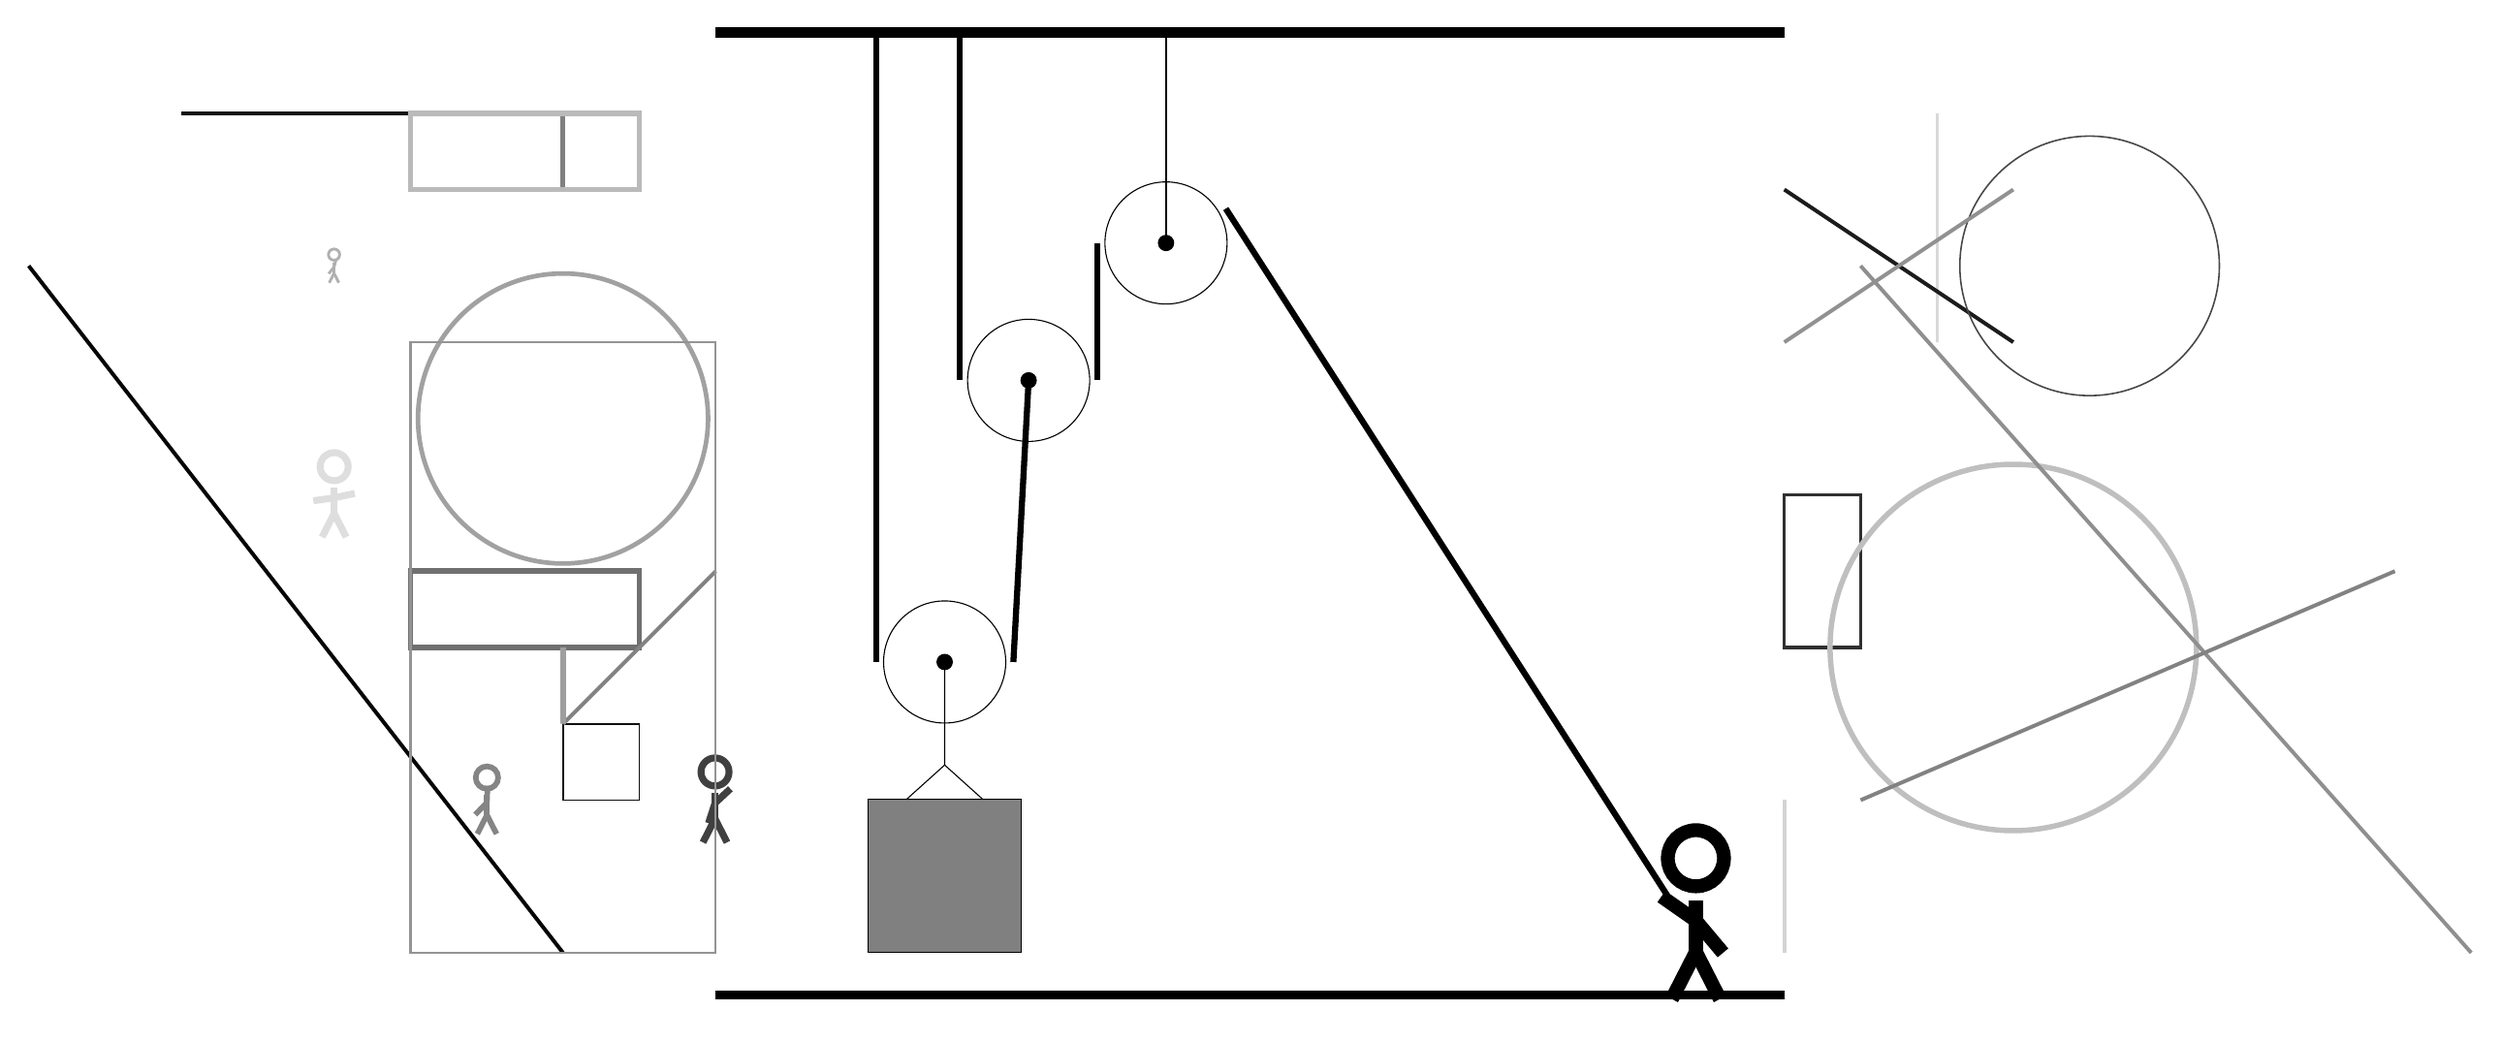
\begin{tikzpicture}
			%%%%% START %%%%%
			
			\draw[fill=black] (-2, 9) rectangle (12, 9.125);
			
			\draw (1, 0.81) circle (0.8);
			\draw[fill=black] (1, 0.81) circle (0.1);
			
			\draw (2.1, 4.5) circle (0.8);
			\draw[fill=black] (2.1, 4.5) circle (0.1);
			
			\node[line width=0.3mm, color=black!48] at (-5, -1) {\Strichmaxerl[4][46][88]};
			
			\node[line width=0.5mm, color=black!31] at (-7, 6) {\Strichmaxerl[2][51][75]};
			\draw[line width=0.6mm, color=black!50] (-4, 8) rectangle (-6, 7);
			\draw[line width=0.4mm, color=black!81] (12, 1) rectangle (13, 3);
			
			\draw [line width=0.7mm, color=black!25](15, 1) circle (2.4);
			\draw[line width=0.4mm, color=black!15] (14, 8) rectangle (14, 5);
			
			\draw[line width=0.5mm, color=black!98](-4, -3) -- (-11, 6);
			
			\draw[line width=0.7mm, color=black!56] (-3, 2) rectangle (-6, 1);
			\draw[line width=0.2mm, color=black!94] (-4, -1) rectangle (-3, 0);
			\draw[line width=0.5mm, color=black!44](13, 6) -- (21, -3);
			\draw[line width=0.5mm, color=black!89](15, 5) -- (12, 7);
			\node[line width=0.6mm, color=black!13] at (-7, 3) {\Strichmaxerl[5][8][12]};
			\draw[line width=0.5mm, color=black!49](-4, 0) -- (-2, 2);
			
			\draw [line width=0.2mm, color=black!72](16, 6) circle (1.7);
			\draw[line width=0.5mm, color=black!93](-4, 8) -- (-9, 8);
			\draw[line width=0.5mm, color=black!17](12, -1) -- (12, -3);
			
			\node[line width=0.4mm, color=black!75] at (-2, -1) {\Strichmaxerl[5][72][43]};
			
			\draw[line width=0.5mm, color=black!43](12, 5) -- (15, 7);
			\draw [line width=0.6mm, color=black!37](-4, 4) circle (1.9);
			\draw[line width=0.3mm, color=black!42] (-2, 5) rectangle (-6, -3);
			\draw[line width=0.7mm, color=black!27] (-3, 8) rectangle (-6, 7);
			
			\draw[line width=0.5mm, color=black!49](13, -1) -- (20, 2);
			
			\draw[line width=0.7mm, color=black!38] (-4, 0) rectangle (-4, 1);
			
			\draw (3.9, 6.3) circle (0.8);
			\draw[fill=black] (3.9, 6.3) circle (0.1);
			\draw[thick] (3.9, 6.3) -- (3.9, 9);
			
			\draw (1, 0.81) -- (1, -0.54) -- (0.5, -0.99) -- (1.5, -0.99) -- (1, -0.54);
			\draw[fill=black!50] (0, -0.99) rectangle (2, -2.99);
			
			\draw[line width=0.8mm] (0.1, 9) -- (0.1, 0.81);
			\centerarc[line width=0.8mm](1, 0.81)(180:360:0.9);
			\draw[line width=0.8mm](1.9, 0.81) -- (2.1, 4.5);
			\draw[line width=0.8mm] (1.2, 9) -- (1.2, 4.5);
			\centerarc[line width=0.8mm](2.1, 4.5)(180:360:0.9);
			\draw[line width=0.8mm](3.0, 4.5) -- (3.0, 6.3);
			\centerarc[line width=0.8mm](3.9, 6.3)(30:180:0.9);
			\draw[line width=0.8mm] (4.683, 6.75) -- (10.5, -2.3);
			
			\node at (10.8, -2.5) {\Strichmaxerl[10][-35][-50]};
			
			\draw[fill=black] (-2, -3.5) rectangle (12, -3.6);
			
			%%%%% END %%%%%
		\end{tikzpicture}
	\end{figure}	
\end{document}